%%%%%%%%%%%%%%%%%%%%%%%%%%%%
%%%%%%%%%%%%%%%%%%%%%%%%%%%%
\section{Confidence Sets} \label{sec:confidence}

Boostrap, jackknife and bayesian estimation naturally produce a forest of trees with the same species set. But different trees can also be estimated using different methods or different sources of data. One way to summarize the forest is to \emph{project} it on a focal tree to compute support values (see section~\ref{sec:robustness}). Alternatively, one can bypass the focal tree and combine all trees in the forest to get a single tree. That is the purpose of consensus trees methods. 

%%%%%%%%%%%%%%%%%%%%%%%%%%%%
\subsection{Consensus Tree} \label{sec:consensus-tree}

\emph{Consensus trees} are trees that summarize a forest of trees with the same species set. We present here only the \emph{strict} consensus, the \emph{majority rule} consensus and the \emph{extended majority rule} consensus but there are many other consensus (see \citet{Bryant2003} for an extensive survey). The different notions are best understood on an example and we'll refer to Figure~\ref{fig:consensus} throughout the discussion. 

\begin{figure}
 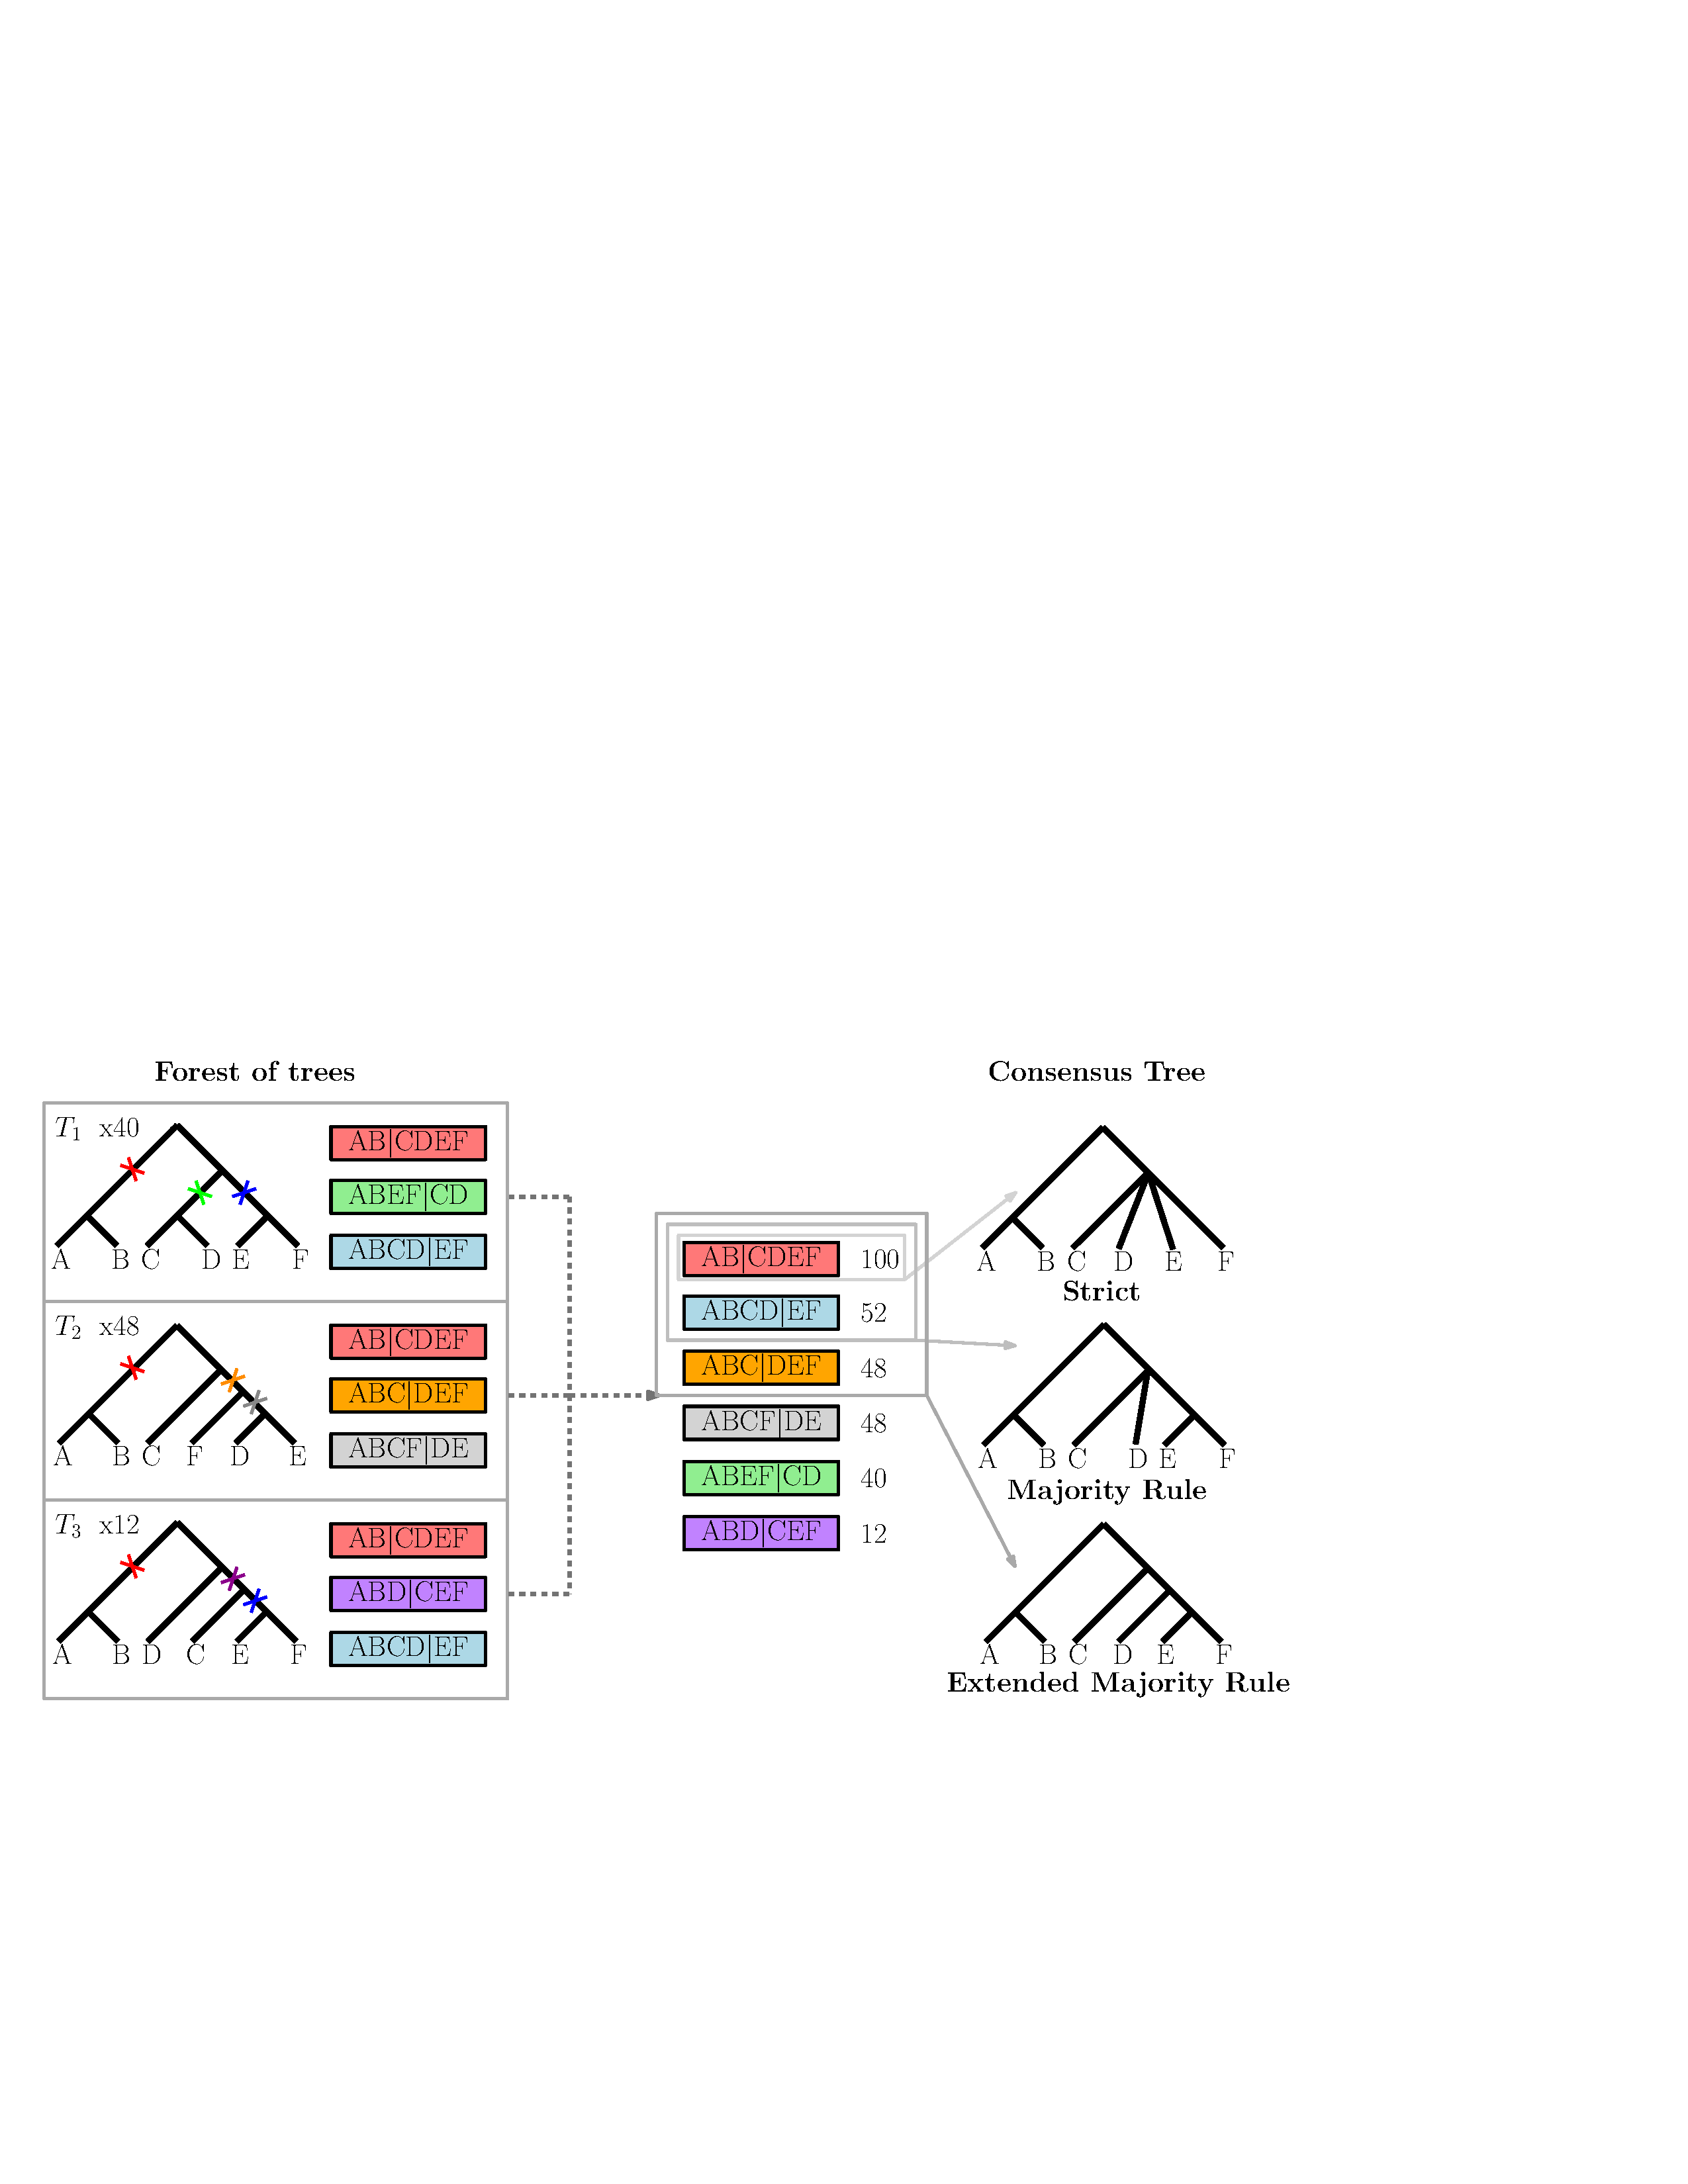
\includegraphics[width=0.9\linewidth]{Figs/consensus}
 \caption{Left: a forest of $100$ trees made of $3$ topologies. Middle: Set of all bipartitions, with their frequencies found in the forest. Right: Different consensus made up by increasing large sets of partitions.}
 \label{fig:consensus}
\end{figure}

%%%%%%%%%%%%%%%%%%%%%%%%%%%%
\subsubsection{}



Different methods for a consensus (and problems in terms of branch lengths reconstruction)

%%%%%%%%%%%%%%%%%%%%%%%%%%%%
\subsection{Confidence Set} \label{sec:confidence-sets}

Easy to understand in a Bayesian setting, a bit more involved (AIC weights) in a frequentist framework. 
